\documentclass{beamer}
\usetheme{Berlin}
\setbeamercovered{dynamic}
\title[Beamer]{Beamer}
\subtitle{Lab Quiz}
\author{Tanishq Trivedi}
\date{\today}
\institute{IIT Dharwad}

\begin{document}

\begin{frame}
\titlepage
\begin{figure}
\centering
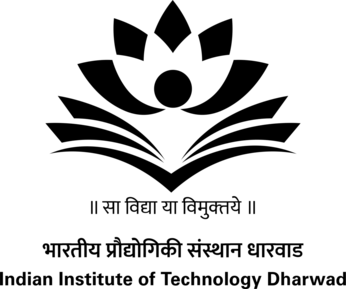
\includegraphics[scale=0.25]{iitdhlogo}
\end{figure}
\end{frame}

\begin{frame}
\frametitle{Contents}
\tableofcontents
\end{frame}

\section{Synchronised Display}

\begin{frame}
\frametitle{Synchronised Display}
\begin{columns}
	\begin{column}{.45\textwidth}
		\begin{alertblock}{Row-wise table display}
		
\begin{tabular}{lcccc}
  \uncover<1-5>{Class & A & B & C & D} \\
  \uncover<2-5>{X     & 1 & 2 & 3 & 4} \\
  \uncover<3-5>{Y     & 3 & 4 & 5 & 6} \\
  \uncover<4-5>{Z     & 5 & 6 & 7 & 8}
\end{tabular}

		\end{alertblock}

	\end{column}
	\column{.45\textwidth}
	
		\begin{exampleblock}{Column-wise table display}
		
\begin{tabular}{lcccc}
  \uncover<1-5>{Class & A & B & C & D} \\
  \uncover<2-5>{X     & 1 & 2 & 3 & 4} \\
  \uncover<3-5>{Y     & 3 & 4 & 5 & 6} \\
  \uncover<4-5>{Z     & 5 & 6 & 7 & 8}
\end{tabular}

		\end{exampleblock}

\end{columns}

\begin{block}{Mathematics}

\begin{eqnarray*}
2x^2 + 3(x-1)(x-2) \pause &=&2x^2 + 3(x^2-3x+2)\\
\pause &=& 2x^2 + 3x^2 - 9x + 6\\
\pause &=& 5x^2 - 9x + 6
\end{eqnarray*} 
\end{block}
\end{frame}

\section{Infinite loop}
\begin{frame}\label{prevslide}

\frametitle{Infinite loop}
\hyperlink{nextslide}{\beamergotobutton{Go to next slide}}
\end{frame}

\begin{frame}\label{nextslide}

\frametitle{Infinite loop}
\hyperlink{prevslide}{\beamergotobutton{Go to previous slide}}

\end{frame}

\section{Conclusion}
\begin{frame}
\centering
Thank You
\end{frame}

\end{document}